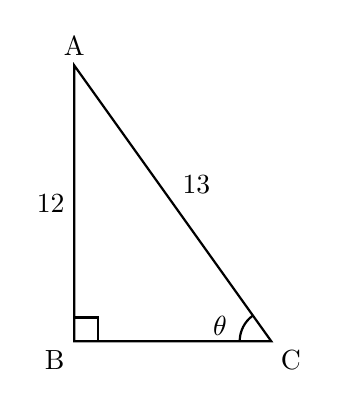
\begin{tikzpicture}[scale=1]

    % Define the vertices of the right-angled triangle
    % The coordinates are chosen to maintain the visual proportions of the image
    \coordinate (B) at (0,0);
    \coordinate (C) at (2.5,0);
    \coordinate (A) at (0,3.5);

    % Draw the sides of the triangle
    \draw[thick] (A) -- (B) -- (C) -- cycle;

    % Draw the right-angle square symbol at vertex B
    \draw[thick] (0,0.3) -- (0.3,0.3) -- (0.3,0);

    % Add labels for the vertices A, B, and C
    \node[above] at (A) {A};
    \node[below left] at (B) {B};
    \node[below right] at (C) {C};

    % Add labels for the lengths of the sides
    \node[left] at (0,1.75) {12};
    \node[above right] at (1.25,1.75) {13};

    % Draw the arc for the angle at C
    % The line CA has an angle of approximately 125.5 degrees from the positive x-axis
    % We draw the arc from 180 degrees (line CB) down to 125.5 degrees
    \draw[thick] (C) ++(-0.4,0) arc (180:125.5:0.4);
    
    % Add the angle label theta inside the arc
    \node at (1.85, 0.2) {$\theta$};

\end{tikzpicture}